\documentclass[12pt]{article}
\usepackage[margin=2.5cm]{geometry}
\usepackage{enumerate}
\usepackage{amsfonts}
\usepackage{amsmath}
\usepackage{fancyhdr}
\usepackage{amsmath}
\usepackage{amssymb}
\usepackage{amsthm}
\usepackage{mdframed}
\usepackage{graphicx}
\usepackage{subcaption}
\usepackage{adjustbox}
\usepackage{listings}
\usepackage{xcolor}
\usepackage{booktabs}
\usepackage[utf]{kotex}

\definecolor{codegreen}{rgb}{0,0.6,0}
\definecolor{codegray}{rgb}{0.5,0.5,0.5}
\definecolor{codepurple}{rgb}{0.58,0,0.82}
\definecolor{backcolour}{rgb}{0.95,0.95,0.92}

\lstdefinestyle{mystyle}{
    backgroundcolor=\color{backcolour},
    commentstyle=\color{codegreen},
    keywordstyle=\color{magenta},
    numberstyle=\tiny\color{codegray},
    stringstyle=\color{codepurple},
    basicstyle=\ttfamily\footnotesize,
    breakatwhitespace=false,
    breaklines=true,
    captionpos=b,
    keepspaces=true,
    numbers=left,
    numbersep=5pt,
    showspaces=false,
    showstringspaces=false,
    showtabs=false,
    tabsize=1
}

\lstset{style=mystyle}

\begin{document}
\title{CSC236 Worksheet 8 Solution}
\author{Hyungmo Gu}
\maketitle

\section*{Question 1}

\bigskip

\underline{\textbf{Notes:}}

\bigskip

\begin{itemize}
    \item \textbf{Deterministic Finite State Automaton (DFSA)}: is a mathematical
    method of machine which, given any input string $x$, \textbf{accepts} or
    \textbf{rejects} $x$.

    \item Applications of DFSA
    \begin{enumerate}[1.]
        \item Vending Machine
        \begin{center}
        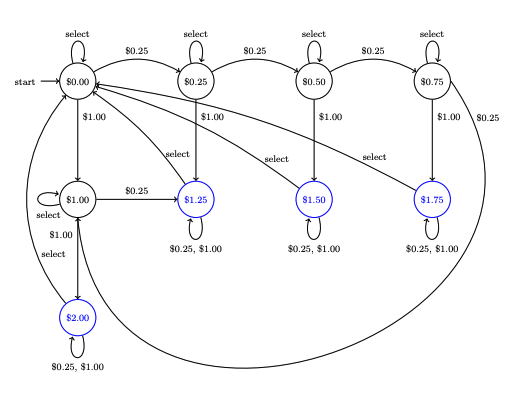
\includegraphics[width=0.8 \linewidth]{images/worksheet_8_notes_1.png}
        \end{center}

        \item Protocol analysis
        \item Text parsing
        \item Video game character behavior

        \begin{center}
        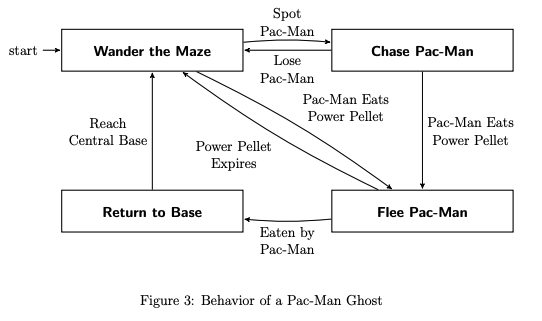
\includegraphics[width=0.8 \linewidth]{images/worksheet_8_notes_2.png}
        \end{center}

        \item Security Analysis
        \item \underline{CPU control units} (**)
        \item \underline{Natural Language Processing} (**)
        \item \underline{Speech Recognition}  (**)
    \end{enumerate}

    \item Definitions and Syntax
    \begin{center}
    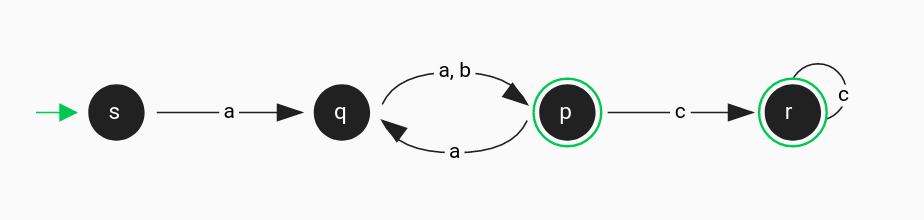
\includegraphics[width=\linewidth]{images/worksheet_8_notes_6.png}
    \end{center}
    \begin{itemize}
        \item $DFSA$ $M$ is a quintuple $M = (Q,\Sigma, q_0, F, \delta)$, where
        \begin{itemize}
            \item $Q:$ a finite set of \textbf{states}.
            \begin{itemize}
                \item Represents status of system
                \item Is represented by a black circle, i.e. s,q

                \begin{center}
                
\includegraphics[width=2cm]{images/worksheet_8_notes_8.png}
                \end{center}

                \item i.e. automatic sliding door at walmart has two states: either close or open
                \item i.e. traffic light has three states: red, yellow, green
            \end{itemize}
            \item $\Sigma:$ a finite non-empty alphabet
            \begin{itemize}
                \item is set of symbols in each transition, i.e. a, b, c

                \begin{center}
                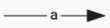
\includegraphics[width=0.3 \linewidth]{images/worksheet_8_notes_3.png}
                \end{center}
            \end{itemize}

            \item $q_0 \in Q:$ the start or initial state
            \item $\delta: Q \times \sigma \to Q:$ a transition function
            \begin{itemize}
                \item is a connection between two states.
                \item is represented by an arrow
                \begin{center}
                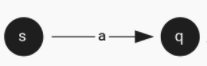
\includegraphics[width=0.4 \linewidth]{images/worksheet_8_notes_4.png}
                \end{center}
            \end{itemize}
            \item $F \subseteq Q:$ the set of accepting or final states
            \begin{itemize}
                \item Is represented by a double circle

                \begin{center}
                
\includegraphics[width=2cm]{images/worksheet_8_notes_5.png}
                \end{center}

                \item Multiple accepting states may exists
                \item Purpose: When processing ends, the output is either \textit{accept} or \textit{reject}
            \end{itemize}
        \end{itemize}
    \end{itemize}

    \item Simple Example

    \begin{itemize}
        \item

        \begin{center}
        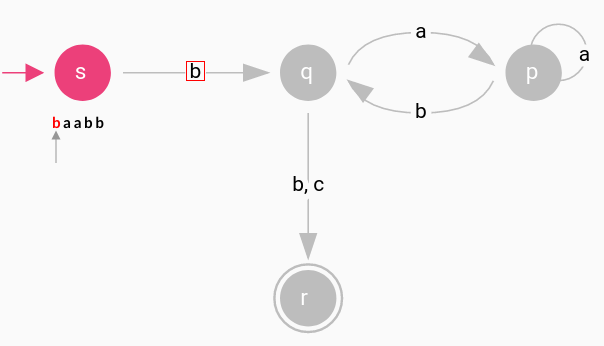
\includegraphics[width=\linewidth]{images/worksheet_8_notes_9.png}
        \end{center}
    \end{itemize}
\end{itemize}

\end{document}